

% trial .tex file %
\documentclass[9pt]{article}  % specifies document class (article) and point size (10pt)
\usepackage{graphicx}
\usepackage{polski}
\usepackage[utf8]{inputenc}
\usepackage{sidecap}
\usepackage{wrapfig}
\usepackage{subfig}
\usepackage{amsmath}
\usepackage{float}
\usepackage{enumerate}
\usepackage{listings}
\usepackage{listings}
\usepackage{color}

\definecolor{dkgreen}{rgb}{0,0.6,0}
\definecolor{gray}{rgb}{0.5,0.5,0.5}
\definecolor{mauve}{rgb}{0.58,0,0.82}

\lstset{frame=tb,
  language=R,
  aboveskip=3mm,
  belowskip=3mm,
  showstringspaces=false,
  columns=flexible,
  basicstyle={\small\ttfamily},
  numbers=none,
  numberstyle=\tiny\color{gray},
  keywordstyle=\color{blue},
  commentstyle=\color{dkgreen},
  stringstyle=\color{mauve},
  breaklines=true,
  breakatwhitespace=true,
  tabsize=3
}


\begin{document}               % starts document
\author{Michał Kubica}
\title{Modele Liniowe \\ Raport nr 2}       
\maketitle                     % constructs big, fancy title

\section{Zadanie 1}            % makes a section header

    \begin{figure}[H]
      \centering
      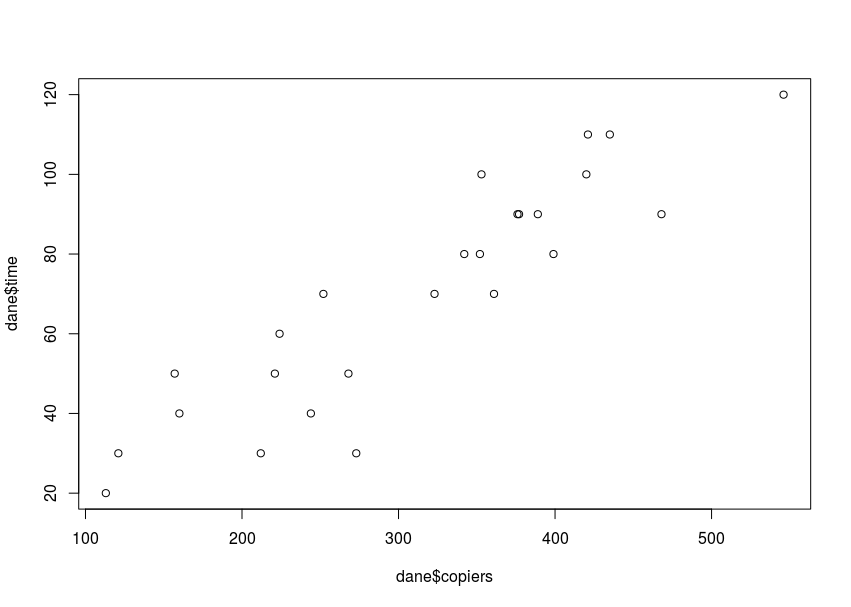
\includegraphics[width=1\textwidth]{1.png}
      \caption {Zależność czasu obsługi od ilości kopiarek}
    \end{figure} 

  Widać, że w przybliżeniu relacja jest liniowa.
  

    \begin{lstlisting}
    plot(dane$copiers,dane$time)
    \end{lstlisting}  

    
\section{Zadanie 2}

  \begin{enumerate}[a)]
    \item Wyestymowane równanie regresji liniowej za pomocą funkcji \textit{lm} \newline
    $ Y = 0.2301084 \cdot X - 1.8582511$ \newline
    Na podstawie wzorów (1) i (2) upewniono się, że równanie regresji zostało obliczone poprawnie.
    \item 95\% przedział ufności dla współczynnika kierunkowego.  \newline
    Wyliczony przedział ufności za pomocą funkcji \textit{confint}: \newline
    (0.1838466, 0.2763702) 
    \item Testowanie \newline
    $H_0$ : nie ma zależnosci liniowej, współczynnik korelacji jest równy 0 \newline
    Na podstawie małej p wartości równej $4.448828 \cdot 10^{-10}$, możemy odrzucić hipotezę zerową. A więc w podanym zbiorze danych zaobserwujemy zależność liniową. \newline
    
    
    \begin{lstlisting}
    m1 = lm(dane$time~dane$copiers)
    confint(m1, level=0.95)
    b1 = (sum((dane$copiers-mean(dane$copiers))*(dane$time - mean(dane$time) ) )) / sum( (dane$copiers-mean(dane$copiers))^2 )
    b0 = mean(dane$time) - b1*mean(dane$copiers)
    summary(m1)
    \end{lstlisting}  

  \end{enumerate}


  \begin{equation}
  b_1 = \frac{\sum{\left(X_i - \bar{X} \right) \left( Y_i - \bar{Y} \right) } }{\sum{\left(X_i - \bar{X} \right) ^2 } }
  \end{equation}

  \begin{equation}
  b_0 = \bar{Y} - b_1 \bar{X}
  \end{equation}

\section{Zadanie 3}

  Najpierw wyznaczono
  
  $$\hat{Y_i}  =b_0 +b_1 X_i$$
  
  Następnie wyliczono estymator wariancji
  
  $$ s^2 = \frac{ \sum{ \left( Y_i - \hat{Y_i} \right)^2 } } { n-2 } = 153.6364$$

  Oraz estymator wartości oczekiwanej dla $X_h = 11$

  $$ \hat{\mu}_h = b_0 + b_1 X_h = 0.6729413$$
  
  I estymator wariancji wartości oczekiwanej 
  
  $$ s^2( \hat{\mu}_h ) = s^2 \left[  \frac{1}{n} + \frac{(X_h-\bar{X})^2 }{\sum{(X_i-\bar{X})^2} }   \right] = 205.177$$
  
  Otrzymano przedział ufności ze wzoru

  $$ \hat{\mu}_h \pm t_c s( \hat{\mu}_h )   $$
  
  gdzie $t_c(0.975,23)$ w naszym przypadku wynosi 2.069 \newline
  
  $0.6729413 \pm 14.85372 $

    \begin{lstlisting}
b1 = (sum((dane$copiers-mean(dane$copiers))*(dane$time - mean(dane$time) ) )) / sum( (dane$copiers-mean(dane$copiers))^2 )
b0 = mean(dane$time) - b1*mean(dane$copiers)

Yi = b0+b1*dane$copiers
s = sqrt( sum( (dane$time-Yi)^2  ) / 23 )

est_odch = s^2*(1+ 1/25 + (x-mean(dane$copiers))^2 / sum( (dane$copiers-mean(dane$copiers))^2 ))
b0+b1*x - 2.069*sqrt(est_odch)
b0+b1*x + 2.069*sqrt(est_odch)
    \end{lstlisting}  



\section{Zadanie 4}

Korzystając z funkcji \textit{predict} oraz wzorów ze strony prof. Małgorzaty Bogdan (3) wyznaczono prognozę czasu serwisowania 11 kopiarek oraz 95\% ufności.
\begin{equation}
 s^2( \hat{\mu}_h ) = s^2 \left[  1+ \frac{1}{n} + \frac{(X_h-\bar{X})^2 }{\sum{(X_i-\bar{X})^2} }   \right]
\end{equation}

$0.6729413 \pm 29.63636$


\section{Zadanie 5}
    

 
    \begin{figure}[H]
      \centering
      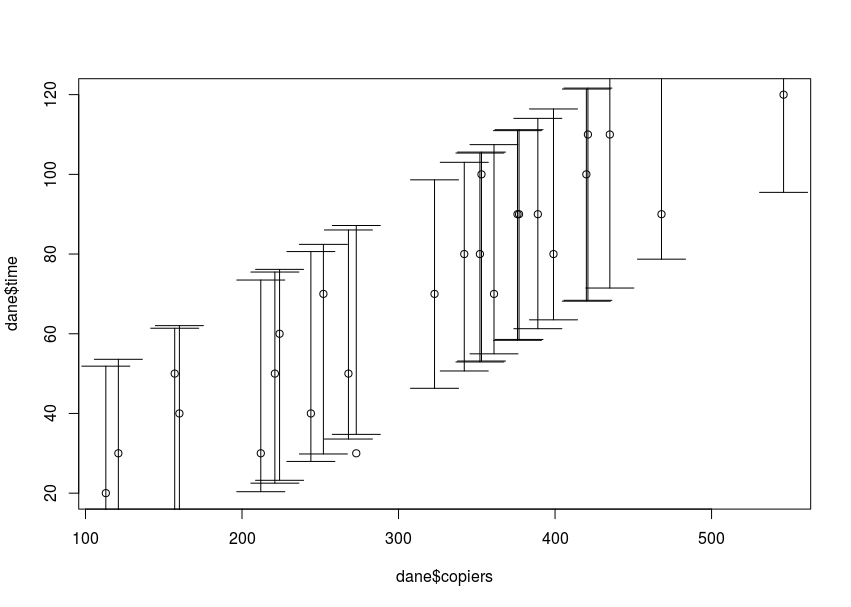
\includegraphics[width=1.2\textwidth]{5.png}
      \caption {}
    \end{figure} 

    


    
    




\end{document}  







